\documentclass{pset}

\usepackage{amsmath}

\usepackage{tikz}
\usetikzlibrary{positioning}
\usetikzlibrary{shapes.arrows}

\newcommand{\TODO}[1]{\textbf{TODO: } #1}

\psnum{3}
\softdue{3/26/15 11:59pm}
\harddue{3/28/15 1:00pm}
\versionnumber{0}

\begin{document}
\maketitle

\section*{Overview}

In this assignment you will implement several functions over infinite streams
of data, an algorithm for inferring types, and an interpreter for OCalf - a
functional language containing the core features of OCaml.

\section*{Objectives}

This assignment should help you develop the following skills:

\begin{itemize}
\item Developing software with a partner.
\item Working with a larger OCaml source code base.
\item Using software development tools like source control.
\item Understanding the environment model and type inference.
\item Experience with infinite data structures and lazy evaluation.
\end{itemize}

\section*{Additional references}

The following supplementary materials may be helpful in completing this assignment:
\begin{itemize}
\item{} Lectures
    \href{http://www.cs.cornell.edu/courses/cs3110/2015sp/lectures/7/lec07.pdf}
    {7},
    \href{http://www.cs.cornell.edu/courses/cs3110/2015sp/lectures/8/lec08.pdf}
    {8}
\item{} Recitations
    \href{http://www.cs.cornell.edu/courses/cs3110/2015sp/recitations/7/rec07.php}
    {7},
    \href{http://www.cs.cornell.edu/courses/cs3110/2015sp/recitations/8/rec08.php}
    {8}
\item{} The \href{http://caml.inria.fr/pub/docs/manual-ocaml/libref/List.html}
    {OCaml List Module} and the
    \href{http://caml.inria.fr/pub/docs/manual-ocaml/libref/Printf.html}
    {Printf Module}
\item{} \href{https://git-scm.com/docs/gittutorial}{Git Tutorial}
\item{} \href{https://realworldocaml.org/v1/en/html/index.html}{Real World OCaml, Chapter 6} 
\end{itemize}

\section*{Academic integrity}

You are allowed to work with one other student in this class for this
problem set. The sharing of code is only allowed between you and your partner;
sharing code among groups is strictly prohibited. Please review the
\link{http://www.cs.cornell.edu/Courses/cs3110/2015sp/syllabus.php\#academic_integrity}{course policy} on academic integrity.

%%%%%%%%%%%%%%%%%%%%%%%%%%%%%%%%%%%%%%%%%%%%%%%%%%%%%%%%%%%%%%%%%%%%%%%%%%%%%%%%

\section*{Provided code}

This is a larger project than those you have worked on in PS1 and 2.  Here is
an overview of the release code.  We strongly encourage you to \textbf{read all
of the \filename{.mli} files before you start coding}, so that you know what
functions are available and understand the structure of the source code.

Here is a brief list of the provided modules:
\begin{description}
\item[Streams] is the skeleton code for part \ref{part:streams}.
\item[Eval and Infer]  are the skeleton code for parts \ref{part:eval} and \ref{part:infer}.
  In addition to the functions that you must implement, there are various
  unimplemented helper functions defined in the \code{.ml} files.  We found
  these helper functions useful when we implemented the assignment, but you
  should feel free to implement them, change them, extend them, or remove them.
  They will not be tested.
\item[Printer] contains functions for printing out values of various
  types.  This will be extremely helpful for testing and debugging.
\item[Examples and Meta] These modules contain example values to help you start
  testing.  \code{Examples} contains all of the examples from this document;
  \code{Meta} contains an extended example for parts \ref{part:eval} and \ref{part:infer}.
\item[Ast and TypedAst] These modules contain the type definitions for parts \ref{part:eval}
  and \ref{part:infer} respectively.  The \code{TypedAst} module also contains the
  \code{annotate} and \code{strip} function for converting between the two.
\item[Parser] contains \code{parse} functions that allow you to read values from
  strings.  It will be useful for testing and debugging parts \ref{part:eval} and \ref{part:infer}.
\end{description}

\section*{Running your code}

In addition to using \texttt{cs3110 test} to test your code, we expect you to
interact extensively with your code in the toplevel.  To support this, we have
provided a \code{.ocamlinit} file%
\footnote{Note that on Linux, files whose names start with `.' are hidden; use
          \texttt{ls -A} to include them in a directory listing.}%
that automatically makes all of your compiled modules available in the
toplevel.  For convenience, it also \code{open}s many of them.

A \code{.ocamlinit} file is just an OCaml file that is automatically
\code{#use}d by the toplevel when it starts.  We encourage you to add to it; any
time you find yourself typing the same thing into the toplevel more than once,
add it to your \code{.ocamlinit}!

In order for the files to load correctly, \textbf{you must compile them first}.
If you change them, the \textbf{changes will not be reflected in the toplevel
until you recompile}, even if you restart it.  The file \filename{examples.ml}
references all other files in the project, so you should be able to recompile
everything by simply running \texttt{cs3110 compile examples.ml}.

\newpage{}
\part{Source control}{5}
\label{part:git}

\textbf{You are required to use some version control system for this project.} We
recommend using \code{git}. As part of good software engineering practices, you should
use version control from the very beginning of the project.
For a tutorial on \code{git}, see the git tutorial in the additional
references section.

You will submit your version control logs in the file \filename{logs.txt}.  These can be
extracted from git by running ``\code{git log --stat > logs.txt}'' at the
command line.

%%%%%%%%%%%%%%%%%%%%%%%%%%%%%%%%%%%%%%%%%%%%%%%%%%%%%%%%%%%%%%%%%%%%%%%%%%%%%%%%

\part{Lazy Evaluation}{30}
\label{part:streams}

A \emph{stream} is an infinite sequence of values. We can model
streams in OCaml using the type
%
\begin{ocaml}
  type 'a stream = Stream of 'a * (unit -> 'a stream)
\end{ocaml}
%
Intuitively, the value of type \code{'a} represents the current
element of the stream and the\\ \code{unit -> 'a stream} is a function
that generates the rest of the stream.

``But wait!'' you might ask, ``why not just use a list?'' It's a good
question. We can create arbitrarily long finite lists in OCaml and we can
even make simple infinite lists. For example:
%
\begin{ocaml}
# let rec sevens = 7 :: sevens;;
val sevens : int list =
  [7; 7; 7; 7; 7; 7; ...]
\end{ocaml}
%
However, there are some issues in using these lists. Long finite lists
must be explicitly represented in memory, even if we only care about a
small piece of them. Also most standard functions will loop forever on infinite
lists:
%
\begin{ocaml}
# let eights = List.rev_map ((+) 1) sevens;;
(loops forever)
\end{ocaml}
%
In contrast, streams provide a compact, and space-efficient way to
represent conceptually infinite sequences of values. The magic happens
in the tail of the stream, which is evaluated lazily---that is, only
when we explicitly ask for it.  Assuming we have a function\\
\code{map_str : ('a -> 'b) -> 'a stream -> 'b stream} that works
analogously to \code{List.map} and a stream \code{sevens_str}, we can
call
\begin{ocaml}
# let eights_str = map_str ((+) 1) sevens_str;;
val eights_str : int stream
\end{ocaml}
and obtain an immediate result. This result is the stream obtained
after applying the map function to the first element of \code{sevens_str}.
Map is applied to the second element only when we ask for the tail of 
this stream.

In general, a function of type \code{(unit -> 'a)} is called a
\emph{thunk}. Conceptually, thunks are expressions whose evaluation
has been delayed. We can explicitly wrap an arbitrary expression (of
type \code{'a}) inside of a thunk to delay its evaluation.  To force
evaluation, we apply the thunk to a unit value. To see how this works,
consider the expression

\begin{ocaml}
  let v = failwith "yolo";;
  Exception: Failure "yolo"
\end{ocaml}
which immediately raises an exception when evaluated. However, if we
write
\begin{ocaml}
  let lazy_v = fun () -> failwith "yolo";;
  val lazy_v : unit -> 'a = <fun>
\end{ocaml}
then no exception is raised. Instead, when the thunk is forced, we see
the error
\begin{ocaml}
  lazy_v ();;
  Exception: Failure "yolo"
\end{ocaml}
In this way, wrapping an expression in a thunk gives rise to
\emph{lazy evaluation}.

\exercise{Implementing Stream Functions (20 points)}

\begin{itemize}
\item[(a)] Implement a function
  \begin{ocaml}
    take : int -> 'a stream -> 'a list
  \end{ocaml}
  that returns the first \code{n} elements of the stream \code{s}
  in a list. If \code{n < 0}, return an empty list.
\item[(b)] Implement a function
  \begin{ocaml}
    repeat : 'a -> 'a stream
  \end{ocaml}
  that produces a stream whose elements are all equal to \code{x}.
\item[(c)] Implement a function
  \begin{ocaml}
    map : ('a -> 'b) -> 'a stream -> 'b stream
  \end{ocaml}
  that (lazily) applies the input function to each element of the
  stream.
\item[(d)] Implement a function
  \begin{ocaml}
    diag : 'a stream stream -> 'a stream
  \end{ocaml}
  that takes a stream of streams of the form
  \[
  \begin{matrix}
    s_{0,0} &  s_{0,1} & s_{0,2} & \cdots \\
    s_{1,0} &  s_{1,1} & s_{1,2} & \cdots \\
    s_{2,0} &  s_{2,1} & s_{2,2} & \cdots \\
    \vdots &  \vdots & \vdots & \ddots
  \end{matrix}
  \]
  and returns the stream containing just the diagonal elements
  \[
  s_{0,0}s_{1,1}s_{2,2}\cdots
  \]
\item[(e)] Implement a function
  \begin{ocaml}
    suffixes : 'a stream -> 'a stream stream
  \end{ocaml}
  that takes a stream of the form 
  \[
  \begin{matrix}
    s_{0} &  s_{1} & s_{2} & s_{3} & s_{4} & \cdots 
  \end{matrix}
  \]
  and returns a stream of streams containing all suffixes of the input
  \[
  \begin{matrix}
    s_{0} &  s_{1} & s_{2} & \cdots \\
    s_{1} &  s_{2} & s_{3} & \cdots \\
    s_{2} &  s_{3} & s_{4} & \cdots \\
    \vdots &  \vdots & \vdots & \ddots
  \end{matrix}
  \]
\item[(f)] Implement a function
  \begin{ocaml}
    interleave : 'a stream -> 'a stream -> 'a stream
  \end{ocaml}
  that takes two streams $s_0s_1\cdots$ and $t_0t_1\cdots$ as input and
  returns the stream
  \[
  s_0t_0s_1t_1s_2t_2\cdots
  \]
\end{itemize}

\exercise{Creating Infinite Streams (10 points)}

In this exercise you will create some interesting infinite
streams. We \emph{highly} recommend using the printing functions we have
provided in \code{printer.ml}. A part of being a good software engineer
is being able to implement tools that will help you test and implement code.
You will have the opportunity to implement your own print function in a later
exercise, but for now, you may use the ones we have provided. See
\code{printer.mli} for more details.

\begin{itemize}
\item[(a)] The Fibonacci numbers $a_i$ can be specified by the recurrence
  relation $a_0 = 0$, $a_1 = 1$, and $a_n = a_{n-1} +
  a_{n-2}$. Create a stream \code{fibs : int stream} whose $n$th
  element is the $n$th Fibonacci number:
  \begin{ocaml}
  print_stream_int (fibs ());;
  [0, 1, 1, 2, 3, 5, 8, 13, ...]
  \end{ocaml}
\item[(b)] The irrational number $\pi$ can be approximated via the formula
  \[
  \pi = 4 \sum_{n=0}^\infty \frac{(-1)^{n}}{2n+1}.
  \]
  Write a stream \code{pi : float stream} whose $n$th element is the
  $n$th partial sum in the formula above:
  \begin{ocaml}
  print_stream_float (pi ());;
  [4., 2.66666666667, 3.46666666667, 2.89523809524,
  3.33968253968, 2.97604617605, 3.28373848374,
  3.017071871707, ...]
  \end{ocaml}
\item[(c)] The \emph{look-and-say sequence} $a_i$ is defined recursively;
  $a_0 = 1$, and $a_n$ is generated from $a_{n-1}$ by reading
  off the digits of $a_{n-1}$ as follows: for each consecutive
  sequence of identical digits, pronounce the number of consecutive
  digits and the digit itself. For example:
  \begin{itemize}
  \item the first element is the number 1,
  \item the second element is 11 because the previous element is read
    as ``one one'',
  \item the third element is 21 because 11 is read as ``two one'',
  \item the fourth element is 1211 because 21 is read as ``one two, one one'',
  \item the fifth element is 111221 because 1211 is read as ``one one,
    one two, two one''.
  \end{itemize}
  Write a stream \code{look_and_say : int list stream} whose $n$th
  element is a list containing the digits of $a_n$ ordered from most
  significant to least significant. Similar to the Fibonacci and pi streams,
  we strongly suggest you test your implementation. To print the
  \emph{look-and-say sequence}, you can use
  \begin{ocaml}
  print_stream_int_list (look_and_say ());;
  [[ 1 ], [ 1 1 ], [ 2 1 ], [ 1 2 1 1 ], [ 1 1 1 2 2 1 ],
  [ 3 1 2 2 1 1 ], [ 1 3 1 1 2 2 2 1 ],
  [ 1 1 1 3 2 1 3 2 1 1 ], ...]
  \end{ocaml}
\end{itemize}

%%%%%%%%%%%%%%%%%%%%%%%%%%%%%%%%%%%%%%%%%%%%%%%%%%%%%%%%%%%%%%%%%%%%%%%%%%%%%%%%

\newpage{}
\part{ML interpreter}{40}
\label{part:eval}

In this part of this assignment, you will implement the evaluation of an
interpreter for a subset of OCaml called OCalf. This will provide
functionality similar to the top-level loop we have been using for much
of the semester.

\section*{Background on interpreters}

An interpreter is a program that takes a source program and computes
the result described by the program. An interpreter differs from a
\emph{compiler} in that it carries out the computations itself rather
than emitting code which implements the specified computation.

\medskip

A typical interpreter is implemented in several \emph{stages}:

\begin{enumerate}
  \item Parsing: the interpreter reads a string containing a program, and
    converts it into a representation called an \emph{abstract syntax tree}
    (AST).  An AST is a convenient data structure for representing programs: it
    is a tree containing a node for each subexpression; the children of the node
    are the subexpressions of the expression.  For example, here is an abstract
    syntax tree representing the program \code{fun x -> 3 + x}:

    \begin{center}
    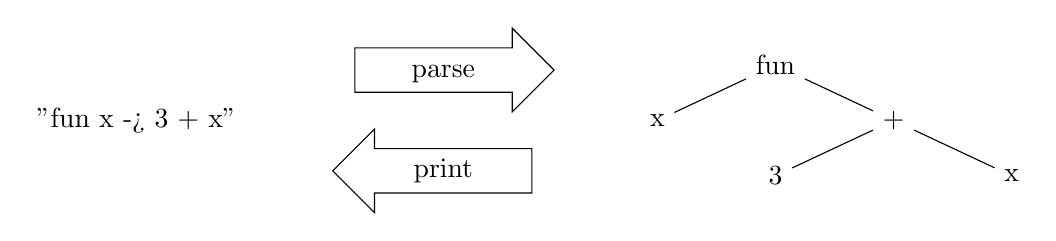
\begin{tikzpicture}
    \node (e) {\code{fun}}
      [sibling distance=3cm,level distance=2em]
      child {node (x) {\code{x}}}
      child {node{\code{+}}
        child {node {\code{3}}}
        child {node {\code{x}}}
      }
    ;
    \node[left = 5cm of x] (prog) {\code{"fun x -> 3 + x"}};
    \path (prog.east) --   node[align=center, text height=.7em, text width=2cm, above=1em,draw,shape=single arrow] {parse} (x)
          (x)         --   node[align=center, text height=.7em, text width=2cm, below=1em,draw,shape=single arrow, shape border rotate=180] {print} (prog.east);
    % \node[left = 1cm of x,draw,shape=single arrow,above,text width=2cm] {parse};
    % \node[left = 1cm of x,draw,shape=single arrow,below] {print};
    \end{tikzpicture}
    \end{center}
    \begin{ocaml}
    utop# parse_expr "fun x -> 3 + x";;
    - : expr = Fun ("x", BinOp (Plus, Int 3, Var "x"))
    \end{ocaml}

  \item Type checking: the interpreter verifies that the program is
    well-formed according to the type system for the
    language---e.g. the program does not contain expressions such as
    \code{3 + true}.
  \item Evaluation: the interpreter evaluates the AST into a final
    \emph{value} (or runs forever).
\end{enumerate}

We have provided you with a type \code{Ast.expr} that represents abstract
syntax trees, as well as a parser that transforms strings into ASTs and a
printer that transforms ASTs into strings. Your task for this part will be to
implement evaluation (typechecking is part \ref{part:infer}).

\section*{Your tasks}

For this part of the assignment, you will be working in the file \code{eval.ml}.
In particular, you will implement the function
  \begin{ocaml}
    eval : Eval.environment -> Ast.expr -> Eval.value
  \end{ocaml}
which evaluates OCalf expressions as prescribed by the
\emph{environment model}.  For example, we can evaluate the expression
``\code{if false then 3 + 5 else 3 * 5}'' in the empty environment as follows:
\begin{ocaml}
eval [] (parse_expr "if false then 3 + 5 else 3 * 5"));;
- : value = VInt 15
\end{ocaml}


\medskip

OCalf has the following kinds of values:
\begin{enumerate}
  \item Unit, integers, booleans, and strings.
  \item Closures, which represent functions and the variables in their scopes.
  \item Variants, which represent user-defined values like \code{Some 3} and \code{None};
        unlike OCaml, all variant values must have an argument.  For example,
        \code{None} and \code{Nil} are represented as \code{None ()} and
        \code{Nil ()}.
  \item Pairs, which represent 2-tuples.  Unlike OCaml, all tuples are pairs;
        you can represent larger tuples as pairs of pairs (e.g.
        \code{(1,(2,3))} instead of \code{(1,2,3)}).
\end{enumerate}

As a simple example of evaluation, using the notation learned in class,
\code{[] :: 7 + 35 || 42}. Your interpreter should evaluate both sides of the
\code{+} operator, which are already values (\code{7} and \code{35}),
and then return an integer representing the sum of values \code{7} and \code{35},
i.e. \code{42}. More details and examples on the environment model can be found in
\link{http://www.cs.cornell.edu/courses/cs3110/2015sp/lectures/7/lec07.pdf}
{the lecture notes}.

Because you can run OCalf programs without type checking them first, your
interpreter may come across expressions it can't evaluate (such as
\code{3 + true} or \code{match 3 with | 1 -> false}).  These expressions should
evaluate to the special value \code{VError}.
  
\exercise{Implement eval without LetRec or Match (30 points)}

We recommend the following plan for this exercise:

\begin{enumerate}
\item[(a)] Implement \code{eval} for the primitive types (\code{Unit},
    \code{Int}, etc.), \code{BinOp} (which represents binary operations like
    \code{+}, \code{*} and \code{^}), \code{If}, \code{Var}, \code{Fun},
    \code{Pair}, and \code{Variant}.
    
    Note: for OCalf, the comparison operators \code{=}, \code{<}, \code{<=},
    \code{>}, \code{>=}, and \code{<>} only operate on integers.
\item[(b)] Implement \code{eval} for \code{App} and \code{Let}.
\end{enumerate}

\exercise{Implement LetRec (5 points)}

Extend \code{eval} to include the evaluation of \code{LetRec}.

Evaluating \code{let rec} expressions is tricky because you need a binding in
the environment for the defined before you can evaluate its definition.  In
lecture we extended the definition of a closure to account for recursive
functions; in this assignment we will use another common technique called
\emph{backpatching}.

To evaluate the expression \code{let rec f = e1 in e2} using backpatching, we
first evaluate \code{e1} in an environment where \code{f} is bound to a dummy
value.  If the value of \code{f} is used while evaluating \code{e1}, it is an
error (this would occur if the programmer wrote \code{let rec x = 3 + x} for
example), however it is likely that \code{e1} will evaluate to a closure that
contains a binding for \code{f} in its environment.

Once we have evalutated \code{e1} to \code{v1}, we imperatively update the
binding of \code{f} within \code{v1} to refer to \code{v1}.  This ``ties the
knot'', allowing \code{v1} to refer to itself.  We then proceed to evaluate
\code{e2} in the environment where \code{f} is bound to \code{v1}.

To support backpatching, we have defined the \code{environment} type to contain
\code{binding ref}s instead of just \code{binding}s.  This enables the bindings
to be imperatively updated.

\exercise{Implement Match (5 points)}

Extend \code{eval} to support \code{match} statements.  Take care to correctly
bind the variables that are defined by the pattern.  You may find it helpful to
implement a function
  \begin{ocaml}
    find_match : pattern -> value -> environment option
  \end{ocaml}
to check for a match and return the bindings if one is found.

If a given match expression does not match any of the patterns in a match
expression, the pattern matching is said to be \emph{inexhaustive}. However,
given pattern matchings, you \textbf{do not need to check if the pattern
matchings are inexhaustive or if there are repetitive match cases.} Your
implementation should return \code{VError} if pattern matching fails at
\emph{run-time}.

\newpage{}
\part{Type inference}{50}
\label{part:infer}

For the third part of the assignment, you will implement type inference for your
interpreted language.  OCaml's type inference algorithm proceeds in three steps.
First, each node of the AST is \emph{annotated} with a different type variable.
Second, the AST is traversed to \emph{collect} a set of equations between types
that must hold for the expression to be well-typed.  Finally, those equations
are solved to find an assignment of types to the original variables (this step
is called \emph{unification}).

For example, suppose we were typechecking the expression \code{(fun x -> 3 + x)}
(this example is \code{infer_example} in the \code{Examples} module of the
provided code).  The annotation phase would add a new type variable to each
subexpression, yielding
\begin{ocaml}
print_aexpr (annotate infer_example);;
  (fun (x:'t04) -> ((x : 't02) + (3 : 't01) :'t03) :'t05)
\end{ocaml}
\begin{center}
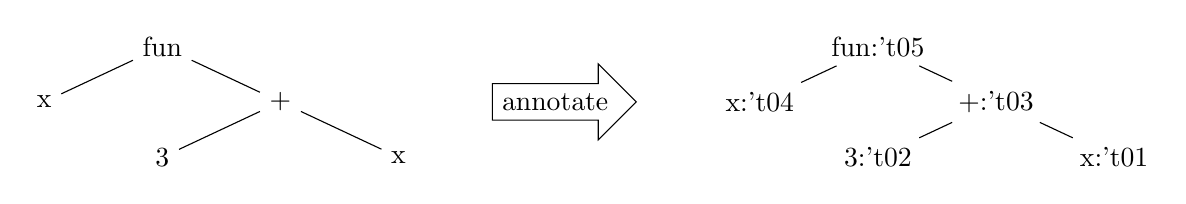
\begin{tikzpicture}
\node (e) {\code{fun}}
  [sibling distance=3cm,level distance=2em]
  child {node{\code{x}}}
  child {node{\code{+}}
    child {node {\code{3}}}
    child {node {\code{x}}}
  }
;
\node[right=8cm of e] {\code{fun:'t05}}
  [sibling distance=3cm,level distance=2em]
  child {node (leftnode) {\code{x:'t04}}}
  child {node{\code{+:'t03}}
    child {node {\code{3:'t02}}}
    child {node {\code{x:'t01}}}
  }
;

\node[left=1cm of leftnode,draw,shape=single arrow] {annotate};

\end{tikzpicture}
\end{center}

Next, we would collect equations from each node.  From our typing rules, we
know that \code{(fun x -> e) : t1 -> t2} if \code{e:t2} under the assumption
\code{x:t1}.  Stated differently, \code{(fun (x:t1) -> e:t2) : t3} if and only
if \code{t3 = t1 -> t2}.  Therefore, while collecting constraints from the
\code{fun} node above, we output the constraint \code{'t05 = 't04 -> 't03}.

Similarly, we must also collect constraints from the \code{+} node.  Our typing
rules tell us that \code{e1 + e2 : int} if and only if \code{e1 : int} and
\code{e2 : int}.  Put another way, \code{(e1:t1) + (e2:t2) : t3} if and only if
\code{t1 = int}, \code{t2 = int}, and \code{t3 = int}.  Therefore, while
collecting constraints from the \code{+} node above, we output the three
equations \code{'t03 = int}, \code{'t02 = int}, and \code{'t01 = int}.

We would also recursively collect the constraints from the \code{3} node and
the \code{x} node.  The rules for typing \code{3} say that \code{3 : t} if and
only if \code{t = int}, so we output the constraint \code{'t02 = int}.  The
rules for variables tell us that if \code{x} had type \code{t} when it was
bound then it has type \code{t} when it is used.  Therefore, when collecting
constraints from the \code{x:'t01} node, we output the equation
\code{'t01 = 't04}.

Putting this together, we have
\begin{ocaml}
print_eqns (collect [] (annotate infer_example));;
      't01 = int              't03 = int
      't02 = int              't04 = 't01
      't02 = int              't05 = 't04 -> 't03
\end{ocaml}

Finally, these equations are solved in the unification step, assigning
\code{int} to \code{'t01} through \code{'t04}, and \code{int->int} to
\code{'t05}.  Substituting this back into the original expression, we have

\begin{ocaml}
print_aexpr (infer [] infer_example);;
  (fun (x:int) -> ((3 : int) + (x : int) :int) : int -> int)
\end{ocaml}

If the constraints output by collect are not satisfiable (for example they may
require \code{int = bool} or \code{'t = 't -> 't}), then it is impossible to
give a type to the expression, so a type error is raised.

If the system is underconstrained, then there will be some unsubstituted
variables left over after the unified variables are plugged in.  In this case,
these variables could have any value, so the typechecker gives them
user-friendly names like \code{'a} and \code{'b}.

\section*{Your type inference tasks}

We have provided the \code{annotate} and \code{unify} phases of type inference
for you; your job is to implement the \code{collect} phase.

\exercise{Implement collect without variants (40 points)}

We recommend the following plan for implementing \code{collect}.

\begin{enumerate}
\item Implement \code{collect} for \code{Fun}, \code{Plus}, \code{Int}, and
  \code{Var}.  This will allow you to typecheck the \code{infer_example}
  example as described above.

\item Implement the \code{collect} function for all syntactic forms
  \emph{except} \code{Variant} and \code{Match}.

\item Implement the \code{collect} function for \code{Match} statements, but
  leave out the handling of \code{PVariant} patterns.  \code{Match} statements
  are a bit trickier because you need to make sure the bindings from the
  patterns are available while checking the bodies of the cases.
\end{enumerate}

\exercise{Implement collect with variants (10 points)}
Extend \code{collect} to handle variant types.  Variant types are
tricky because you need to make use of a type definition to determine how the
types of arguments of a constructor relate to the type that the constructor
belongs to.

Type definitions are represented by \code{TypedAst.variant_spec}s, and a list of
them is provided to the \code{collect} function.  Each variant spec
contains a list \code{vars} of ``free variables'' (like the \code{'a} in
\code{'a last}), a type \code{name} (\code{"list"} in the case of
\code{'a list}), and a list of constructors (with their types).  See
\code{Examples.list_spec} and \code{Examples.option_spec} for examples.

Deriving the correct constraints from a \code{variant_spec} requires some
subtlety.  Consider the following example:
\begin{ocaml}
(Some (1 : t1) : t2, Some ("where" : t3) : t4)
\end{ocaml}
(this is \code{Examples.infer_variant}).  A naive way to typecheck it would be
to collect the constraints \code{'t2 = 'a option} and \code{'t1 = 'a} from
the \code{Some 1} subexpression, and the constraints \code{'t4 = 'a option} and
\code{'t3 = 'a} from the \code{Some "where"} subexpression.

However this would force \code{'a} to be both \code{string} and \code{int}, so
the expression would not typecheck.  A better approach is to think of the
constructor type as a \emph{template} from which you create constraints.  You
can correctly generate the constraints by creating a new type variable for each
of the free variables of the \code{variant_spec}, and substituting them
appropriately in the constructor's type.

In the above example, you might create the variable \code{'x} for \code{'a}
while collecting \code{Some 1}, and output the constraints \code{'t1 = 'x} and
\code{'t2 = 'x option}, and you might create the variable \code{'y} for
\code{'a} while collecting \code{Some "where"}, and output the constraints
\code{'t3 = 'y} and \code{'t4 = 'y option}.  This would allow
\code{infer_variant} to type check correctly.

\exercise{[Optional] Implement let-polymorphism (0 points)}
\textbf{Note:} This question \textbf{is completely optional and will not affect your grade in
any way}.

\textbf{Note 2:} This problem may require you to reorganize your code somewhat.
Make sure you make good use of source control, helper functions, and unit tests
to ensure that you don't break your existing code while working on it!

The type inference algorithm described above allows us to give expressions
polymorphic types: \code{fun x -> x} will be given the type \code{'a -> 'a}.

However, it does not let us use them polymorphically.  Consider the following
expression:
\begin{ocaml}
let (any:t1) = (fun (x:t3) -> (x:t4)):t2 in (any 1, any "where")
\end{ocaml}
(this is \code{Examples.infer_poly}).
OCaml will give this expression the type \code{int * string}, but our naive
inference algorithm fails.

The problem is similar to the subtlety with variants above: we will generate
the constraints \code{(typeof any) = (typeof 1) -> t2}
and \code{(typeof any) = (typeof "where") -> t2}, but these constraints can only
be solved if \code{int = typeof 1 = typeof "where" = string}.

The solution is also similar: every time a variable defined by a \code{let}
expression is used, we create a new type variable corresponding to the use.  We
use the constraints generated while type checking the body of the \code{let} as
a template for a new set of constraints on the new variable.  Using the
constraints from the bodies of lets as templates is called
\emph{let-polymorphism}.

In the above example, while type checking the body of the let expression, we
will generate the constraints \code{t1 = t2}, \code{t2 = t3->t4}, and
\code{t3 = t4}.  While checking the expression \code{(any:t5) 1}, we can
recreate these constraints with new type variables \code{t1'}, \code{t2'}, and
so on.  We will output the constraints \code{t1'=t2'}, \code{t2' = t3'->t4'} and
\code{t3'=t4'}.  We also will output the constraint \code{t5=t1'}.

Because the type variables are cloned, they are free to vary independently.
Because we have cloned their constraints, they must be used in a manner that is
consistent with their definition.

\newpage{}
\part{Written questions}{10}
\label{part:written}

In the file \filename{written.txt} or \filename{written.pdf}, answer the
following questions.

\exercise{Unification (5 points)}
We did not ask you to implement unify, but the algorithm is essentially the
same as the one you use to solve algebraic equations.  To give you a sense of
how it works, solve the following type equations for \code{'t1}, \code{'t2},
and \code{'t3}.

\begin{ocaml}
't5 = 't4 -> 't7              't1 = 't6 -> 't5
't5 = int -> 't6              't2 = 't7 list
't6 = bool                    't3 = bool * 't4
\end{ocaml}

\exercise{Factoring (5 points)}
The type definitions \code{Ast.expr} and \code{TypedAst.annotated_expr} are
nearly identical.  Moreover, there are a number of simple helper functions that
look very similar.

Describe how you might create a single type and helper function that make the
definitions of \code{expr}, \code{annotated_expr}, \code{annotate},
\code{strip}, and \code{subst_expr} all one-liners.

Be sure to make it possible to create an \code{expr} without any
reference to types (that is, don't just define \code{expr} as a synonym for
\code{annotated_expr}).

\exercise{Feedback (0 points)}
Let us know what parts of the assignment you enjoyed, what parts you didn't
enjoy, and any other comments that would help us improve the assignment for the
future.

\section*{What to submit}

You should submit the following files on CMS:
\begin{itemize}
\item{} \filename{streams.ml} containing your stream implementations
\item{} \filename{eval.ml} containing your interpreter
\item{} \filename{infer.ml} containing your type checker
\item{} \filename{written.txt} or \filename{written.pdf} containing your responses to the written questions
\item{} \filename{logs.txt} containing your source control logs
\end{itemize}

\end{document} 

